\chapter{Series}

% ==================================================================================================

\section{Definitions}
\begin{definition}
  A series is defined to be an infinite sum of real numbers:
  \[
    \sum_{i = 1} ^ \infty a_i  
  \]
\end{definition}
This definition isn't very insightful. Instead,
\begin{definition}
  For a series (an infinite series) $\sum_{i = 1} ^ \infty a_i$, the partial sum $S_n$ is defined as
  \[
    S_n = \sum_{i = 1} ^ n a_i  
  \]
\end{definition}
We will use partial sums to define the convergence and divergence of a series.
\begin{definition}
  A sequence converges to some $l \in \R$ if and only if
  \[
    \lim_{n \to \infty} S_n = l  
  \]
  where $(S_n)_{n \geq 1}$ represents the sequence of partial sums.

  A sequence diverges if it does not converge to some $l \in \R$.
\end{definition}
It is very important to note the differences in the definitions of convergence and divergence for sequences and series:

\begin{table}[!htbp]
  \centering
  \begin{tblr}{ccccc}
    \toprule
    Limit & $l \in \R$ & $\infty$ & $-\infty$ & No limit \\
    \midrule
    Sequence $a_n$ & Converges & Converges & Converges & Diverges \\
    Series $\sum a_n$ & Converges & Diverges & Diverges & Diverges \\
    \bottomrule
  \end{tblr}
\end{table}

Nobody knows why we are defining them like this. Anyway, we proceed.

% ==================================================================================================

\section{Tests}
The following section is not strictly laid out according to the slides, but how a student outside of DoC would most likely be learning them.

% --------------------------------------------------------------------------------------------------

\subsection{Divergence test}
\begin{test}[Divergence test]
  \[
    \lim_{n \to \infty} a_n \neq 0 \implies \sumto{n}{\infty} a_n \text{ diverges}
  \]
\end{test}
In the notes, the contrapositive of this test is stated instead (and it is not stated as a test). Note that unlike in sequences, if a series does not diverge, then it converges to some $l \in \R$, which enables this contrapositive statement in the slides. We will prove the contrapositive here.
\begin{proof}
  We want to prove that
  \[
    \sumto{n}{\infty} a_n \text{ converges} \implies \lim_{n \to \infty} a_n = 0
  \]
  Assume $\sumto{n}{\infty} a_n$ converges. Then the sequence $S_n$ converges to some limit $l \in \R$. So $S_n$ is a Cauchy sequence.

  Given some $\epsilon > 0$, using the $\epsilon - N$ definition of convergence, we want find $N \in \N$ such that for all $n > N$, $\abs{a_n} < \epsilon$. Since $S_n$ is a Cauchy sequence,
  \[
    \exists N' \in \N: \forall n, m > N, \abs{S_m - S_n} < \epsilon
  \]
  We pick $m = n + 1$. Then $\abs{S_{n + 1} - S_n} < \epsilon$. Since $S_{n + 1} - S_n = a_{n + 1}$, we have $\abs{a_{n + 1}} < \epsilon$ for all $n > N'$. So let $N = N' + 1$. Then for all $n > N, n - 1 > N'$, so $\abs{a_{n}} < \epsilon$.
\end{proof}

% --------------------------------------------------------------------------------------------------

% Elementary proofs of convergence/divergence of geometric series, harmonic series, etc. here

% --------------------------------------------------------------------------------------------------

\subsection{Comparison test}
We write the following notations:
\begin{itemize}
  \item $\sum_{i = 1} ^ \infty c_i$ represents a (c)onverging series.
  \item $\sum_{i = 1} ^ \infty d_i$ represents a (d)iverging series.
\end{itemize}

\begin{test}[Comparison test]
  If there exists $N \in \N$ such that $\forall i > N$,
  \begin{itemize}
    \item $a_i \leq c_i$, then $\sumto{i}{\infty} a_i$ converges.
    \item $d_i \geq a_i$, then $\sumto{i}{\infty} a_i$ diverges.
  \end{itemize}
\end{test}
Note that there is no need for every term of $a_i \leq c_i$, or $a_i \geq d_i$ -- we just need to show that \textit{after some point}, all terms in the sequence will fulfill the requirement. This enables us to apply the comparison test to determine convergence of series that we would otherwise not be able to determine using the more commonly seen version, which necessitates that \textit{every} term fulfill the requirement.
\begin{eg}
  (MMT 2, 1(b), adapted) Use the comparison test to determine whether the following series converges or diverges:
  \[
    \sumto{n}{\infty} \frac{4}{3n ^ 2 - 4}
  \]
\end{eg}
\begin{solution}
  Let $a_n = \frac{4}{5n ^ 2 - 4}$ and $c_n = \frac{2}{n ^ 2}$.
  \begin{align*}
    a_n \leq c_n &\iff \frac{4}{3n ^ 2 - 4} \leq \frac{2}{n ^ 2} \\
    &\iff 4n ^ 2 \leq 6n ^ 2 - 4 \\ 
    &\iff 2n ^ 2 \geq 4
  \end{align*}
  So $\forall n \geq 2$, $2n ^ 2 \geq 4$, $a_n \leq c_n$.
  \[
    \sumto{n}{\infty} c_n = \sumto{n}{\infty} \frac{2}{n ^ 2} = 2 \sumto{n}{\infty} \frac{1}{n ^ 2}
  \]
  Since $\sum \frac{1}{n ^ 2}$ converges, $\sumto{n}{\infty} c_n$ also converges. So $\sumto{n}{\infty} a_n$ converges.
\end{solution}
\begin{eg}
  (MMT 2, 1(c)) Use the comparison test to determine whether the following series converges or diverges:
  \[
    \sumto{n}{\infty} \frac{1}{n - 4}
  \]
\end{eg}
\begin{solution}
  Let $a_n = \frac{1}{n - 4}$ and $d_n = \frac{1}{n}$.
  \begin{align*}
    d_n \leq a_n &\iff \frac{1}{n} \leq \frac{1}{n - 4} \\ 
    &\iff n - 4 \leq n \\ 
    &\iff -4 \leq 0 \text{ which is true } \forall n.
  \end{align*}
  So $\forall n \geq 1$, $d_n \leq a_n$. Since $d_n$ diverges, $a_n$ diverges.
\end{solution}

% --------------------------------------------------------------------------------------------------

\subsection{Limit comparison test}
\begin{test}[Limit comparison test]
  \begin{align*}
    \lim_{n \to \infty} \frac{a_n}{c_n} = l \in \R &\implies \sumto{n}{\infty} a_n \text{ converges}. \\ 
    \lim_{n \to \infty} \frac{d_n}{a_n} = l \in \R &\implies \sumto{n}{\infty} a_n \text{ diverges}.
  \end{align*}
\end{test}
Note that in this statement of the test, $a_n$ is in the numerator when we want to show convergence, but $a_n$ is in the denominator when we want to show divergence. This is very odd as putting $a_n$ in the denominator does not change anything, but we will accept it for the purposes of passing this module. The more commonly seen version of the test is as follows:
\begin{test}[Limit comparison test, better]
  If $\sumto{n}{\infty} a_n$ and $\sumto{n}{\infty} b_n$ are series such that
  \[
    \lim_{n \to \infty} \frac{a_n}{b_n} = l \in \R
  \]
  then $\sumto{n}{\infty} a_n$ and $\sumto{n}{\infty} b_n$ both converge or both diverge.
\end{test}
\begin{eg}
  (MMT 2, 2(c)) Use the limit comparison test to determine whether the following series converges or diverges:
  \[
    \sumto{n}{\infty} \frac{1}{3n ^ 2 + 4n - 2}
  \]
\end{eg}
\begin{solution}
  Let $a_n = \frac{1}{3n^2 + 4n - 2}$ and $c_n = \frac{1}{3n ^ 2}$.
  \begin{align*}
    \lim_{n \to \infty} \frac{a_n}{c_n} &= \frac{\frac{1}{3n ^ 2 + 4n - 2}}{\frac{1}{3n ^ 2}} \\
    &= \lim_{n \to \infty} \frac{3n ^ 2}{3n ^ 2 + 4n - 2} \\
    &= \lim_{n \to \infty} \frac{3}{3 + \frac{4}{n} - \frac{2}{n ^ 2}} \\
    &= \frac{3}{3 + 0 - 0} \\
    &= 1
  \end{align*}
  Also,
  \[
    \sumto{n}{\infty} c_n = \sumto{n}{\infty} \frac{1}{3n ^ 2} = \frac{1}{3} \sumto{n}{\infty} \frac{1}{n ^ 2}
  \]
  Since $\sumto{n}{\infty} \frac{1}{n ^ 2}$ converges, $\sumto{n}{\infty} c_n$ also converges. Since $\lim_{n \to \infty} \frac{a_n}{c_n} \in \R$ exists and $\sumto{n}{\infty} c_n$ converges, $a_n$ converges.
\end{solution}

% --------------------------------------------------------------------------------------------------

\subsection{D'Alembert's (limit) ratio test}
\begin{test}[D'Alembert's ratio test]
  If there exists some $N \in \N$ such that
  \begin{itemize}
    \item $\frac{a_{n + 1}}{a_n} \geq 1$ for all $n \geq N$, then $\sumto{n}{\infty} a_n$ diverges.
    \item there exists some $k \in \R$ such that $k < 1$ and $\frac{a_{n + 1}}{a_n} \leq k$ for all $n \geq N$, then $\sumto{n}{\infty} a_n$ converges.
  \end{itemize}
\end{test}
This test isn't very useful, but it can be used to prove the correctness of the more useful \textit{limit} ratio test:
\begin{test}[D'Alembert's limit ratio test]
  Suppose $\lim_{n \to \infty} \frac{a_{n + 1}}{a_n} = l \in \R$.
  \begin{itemize}
    \item $l > 1 \implies \sumto{n}{\infty} a_n$ diverges.
    \item $l < 1 \implies \sumto{n}{\infty} a_n$ converges.
    \item $l = 1 \implies$ inconclusive.
  \end{itemize}
\end{test}
For $l = 1$, consider $a_n = \frac{1}{n}$ and $b_n = \frac{1}{n ^ 2}$. The limits $\lim_{n \to \infty} \frac{a_{n + 1}}{a_n}$ and $\lim_{n \to \infty} \frac{b_{n + 1}}{a_b}$ are both 1, but $a_n$ diverges and $b_n$ converges.

Also, it is very painful that we do not introduce the absolute value version (i.e. the correct version) of d'Alembert's (limit) ratio test, since as we will show later, absolute convergence implies unconditional convergence. I am of the strong opinion that this non-absolute value version is wrong, but for the purposes of passing this module, this incorrect version is in this set of notes, as aligned with the slides. The correct version is stated in the next section.
\begin{eg}
  (MMT 2, 3(d)) Using d'Alembert's limit ratio test and $\lim_{n \to \infty} (1 + \frac{1}{n}) ^ n = e$, determine whether the following series converges or diverges:
  \[
    \sumto{n}{\infty} \frac{n!}{n ^ n}
  \]
\end{eg}
\begin{solution}
  Let $a_n = \frac{n!}{n ^ n}$. Since $a_n > 0$ for all $n > 0$, we can apply d'Alembert's limit ratio test.
  \begin{align*}
    \lim_{n \to \infty} \frac{a_{n + 1}}{a_n} &= \lim_{n \to \infty} \frac{(n + 1)!}{(n + 1) ^ {n + 1}} \cdot \frac{n ^ n}{n!} \\ 
    &= \lim_{n \to \infty} \frac{(n + 1)!}{n!} \cdot \frac{n ^ n}{(n + 1) ^ {n + 1}} \\ 
    &= \lim_{n \to \infty} (n + 1) \cdot \frac{n ^ n}{(n + 1) ^ {n + 1}} \\ 
    &= \lim_{n \to \infty} \frac{n ^ n}{(n + 1) ^ n} \\ 
    &= \lim_{n \to \infty} (\frac{n}{n + 1}) ^ n \\ 
    &= \lim_{n \to \infty} \frac{1}{(1 + \frac{1}{n}) ^ n} \\ 
    &= \frac{1}{e} \\ 
    &< 1
  \end{align*}
  So $\sumto{n}{\infty} \frac{n!}{n ^ n}$ converges.
\end{solution}

% --------------------------------------------------------------------------------------------------

\subsection{Integral test}
\begin{test}[Integral test]
  Let $f: \R \to \R$ be continuous, decreasing, and positive on the interval $[1, \infty)$, such that $a_n = f(n)$. If there exists $N \in \N$ such that
  \begin{itemize}
    \item $\int_N^\infty\! f(x) \di x$ converges, then $\sumto{n}{\infty} a_n$ converges.
    \item $\int_N^\infty\! f(x) \di x$ diverges, then $\sumto{n}{\infty} a_n$ diverges.
  \end{itemize}
\end{test}
\begin{eg}
  We consider the upper Riemann approximation to show that $\sumto{n}{\infty} \frac{1}{n}$ diverges.
  \begin{figure}[!htbp]
    \centering
    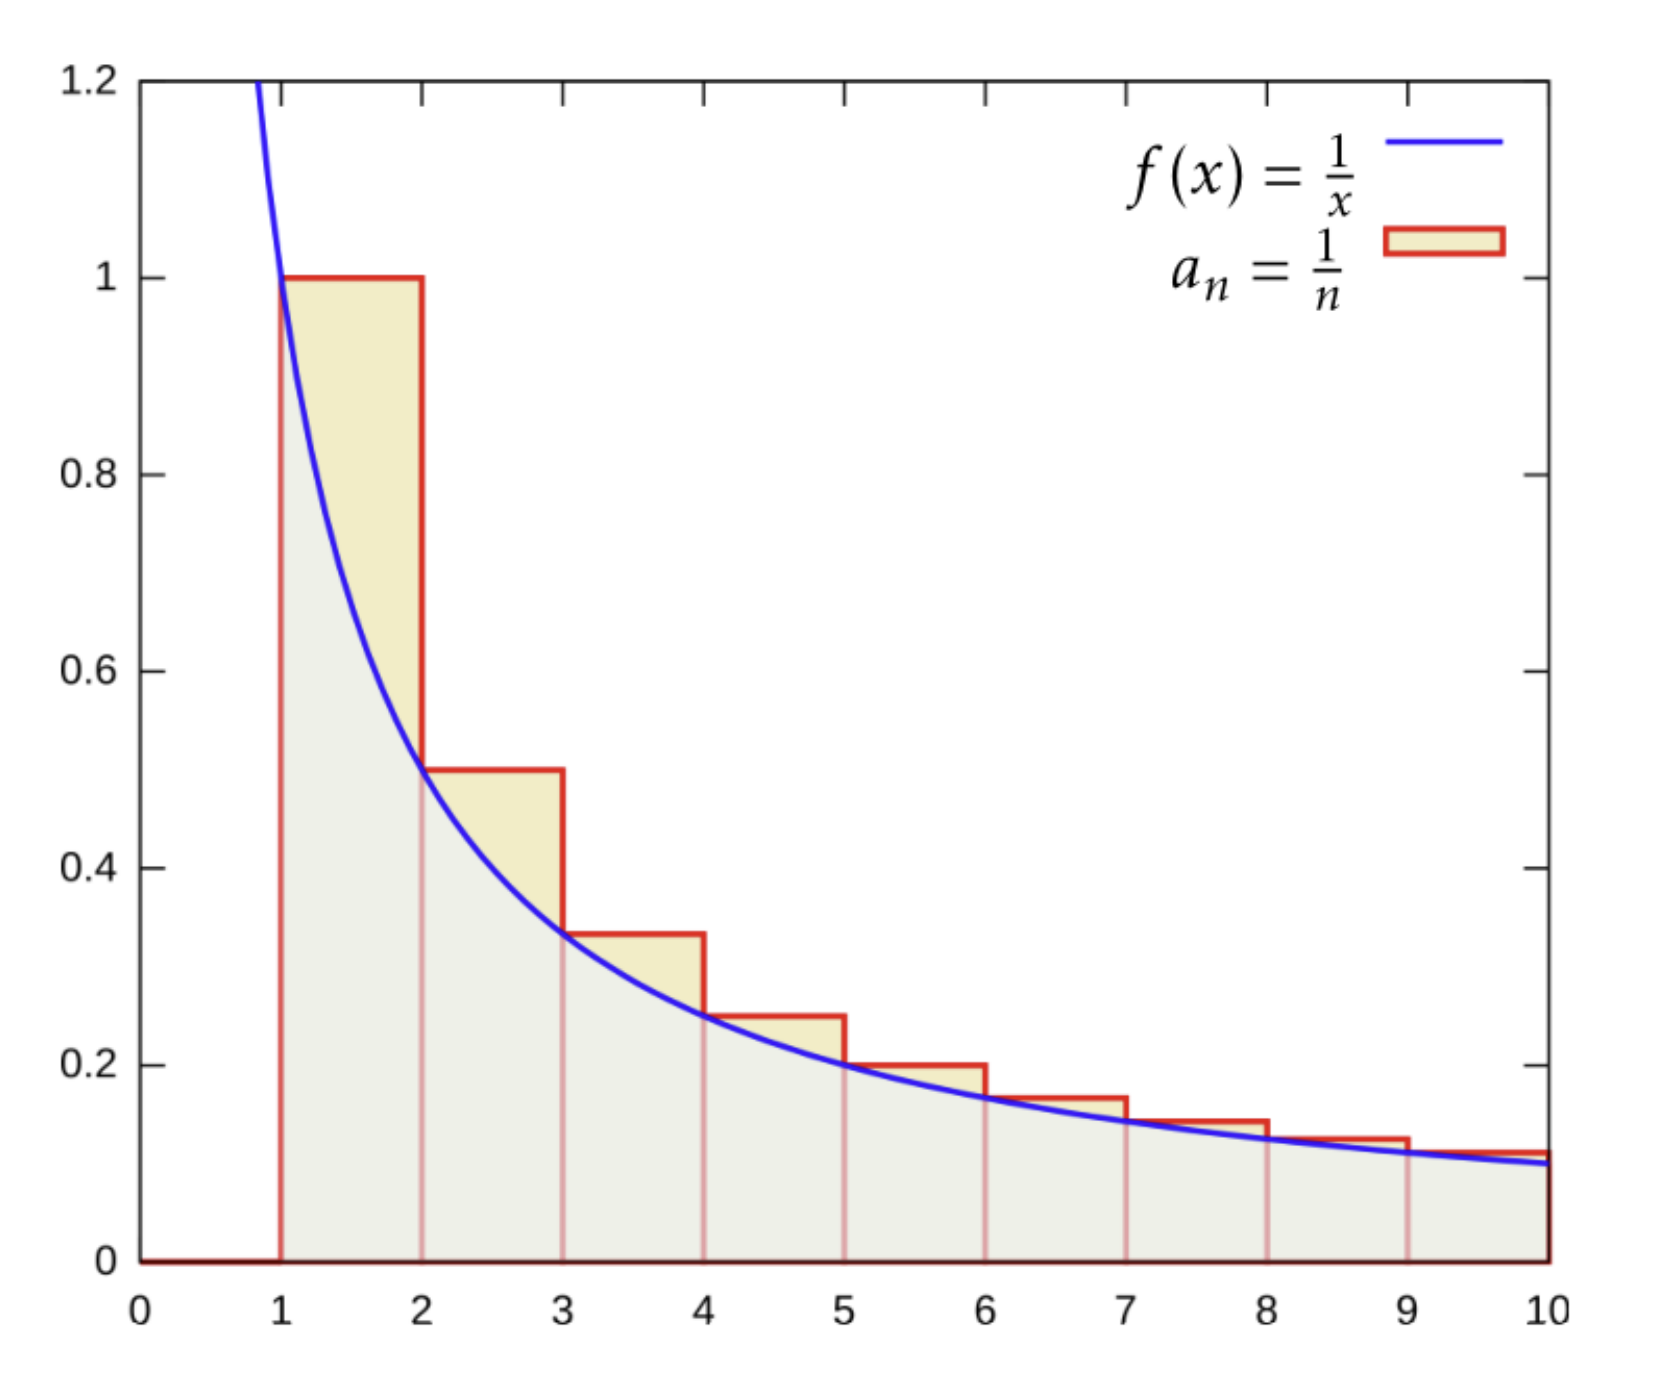
\includegraphics[width=0.6\columnwidth]{week_06_upper}
    \caption{Upper Riemann approximation of $\frac{1}{n}$}
  \end{figure}
  It is clear from the diagram that $\sumto{n}{\infty} \frac{1}{n} > \int_1^{\infty} \frac{1}{n}$. Then,
  \begin{align*}
    \int_1^{\infty}\! \frac{1}{x} \di x &= \lim_{b \to \infty} [\ln x]_1^b \\ 
    &= \lim_{b \to \infty} [\ln b - \ln 1] \\ 
    &= \lim_{b \to \infty} \ln b
  \end{align*}
  which diverges since $\ln x$ is strictly increasing and not bounded above. So $\sumto{n}{\infty} \frac{1}{n}$ also diverges.
\end{eg}
\begin{eg}
  We consider the lower Riemann approximation to show that $\sum_{n = 2}^\infty \frac{1}{n ^ 2}$ converges (note that we are summing from 2, not 1).
  \begin{figure}[!htbp]
    \centering
    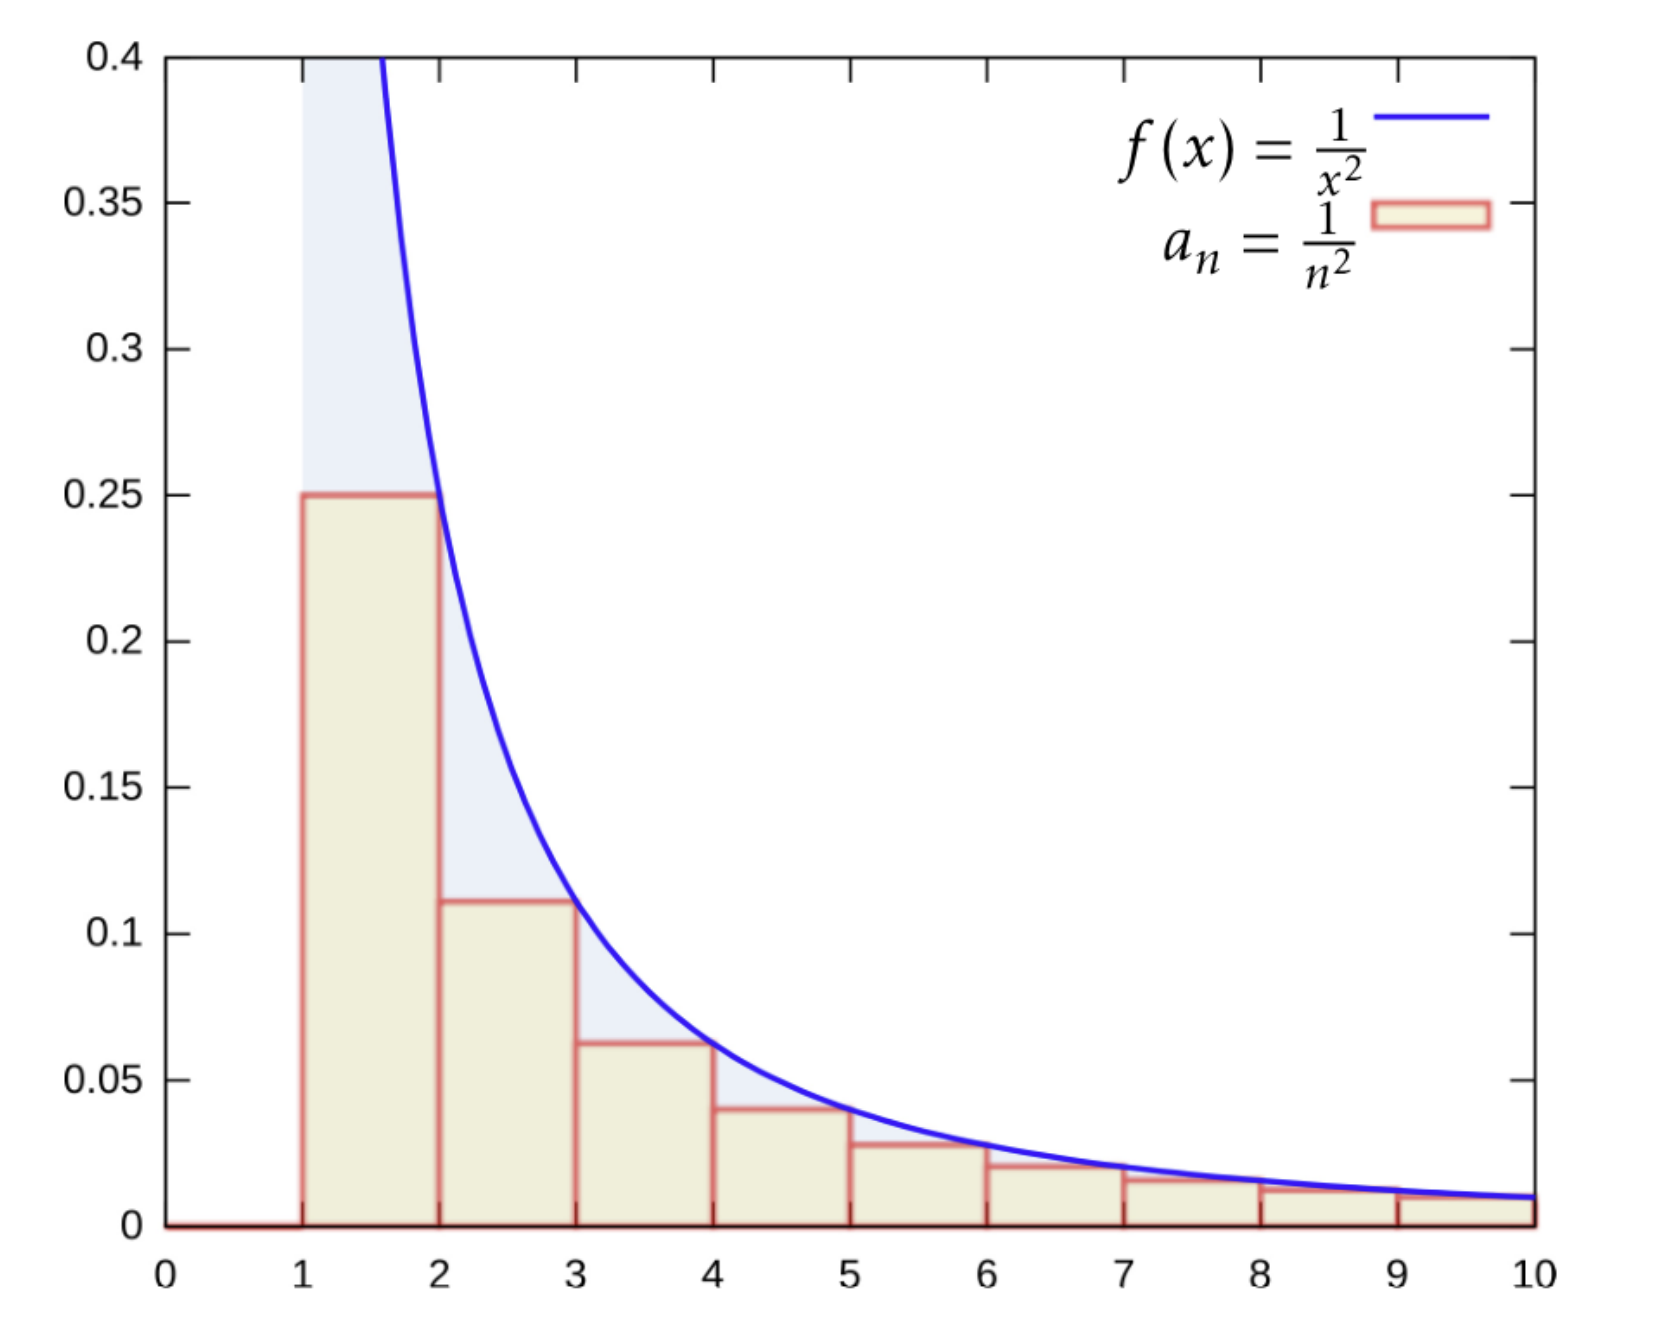
\includegraphics[width=0.6\columnwidth]{week_06_lower}
    \caption{Lower Riemann approximation of $\frac{1}{n ^ 2}$}
  \end{figure}
  It is clear from the diagram that $\sum_{n = 2}^\infty \frac{1}{n} < \int_1^{\infty} \frac{1}{n ^ 2}$. Then,
  \begin{align*}
    \int_1^{\infty}\! \frac{1}{x ^ 2} \di x &= \lim_{b \to \infty} \left[-\frac{1}{x}\right]_1^b \\ 
    &= \lim_{b \to \infty} (-\frac{1}{b} + \frac{1}{1}) \\ 
    &= \lim_{b \to \infty} (1 - \frac{1}{b}) \\ 
    &= 1 - 0 \\ 
    &= 1
  \end{align*}
  so the integral converges. Then $\sum_{n = 2}^\infty \frac{1}{n ^ 2}$ also converges, so $\sum_{n = 1}^\infty \frac{1}{n ^ 2}$ converges.
\end{eg}
\begin{eg}
  (MMT 2, 4) Use the integral test to determine whether the following series converges or diverges:
  \[
    \sumto{n}{\infty} \frac{1}{e ^ n}
  \]
\end{eg}
\begin{solution}
  Let $f(x) = \frac{1}{e ^ x}$. $f(x)$ is continuous, decreasing, and positive on the interval $[1, \infty)$.
  \begin{align*}
    \int_1^\infty\! f(x) \di x &= \lim_{b \to \infty} \int_1^b\! \frac{1}{e ^ x} \di x \\ 
    &= \lim_{b \to \infty} \left[-\frac{1}{e ^ x}\right]_1^b \\ 
    &= \lim_{b \to \infty} (-\frac{1}{e ^ b} + \frac{1}{e}) \\ 
    &= 0 + \frac{1}{e} \\ 
    &= \frac{1}{e}
  \end{align*}
  so the integral converges. So $\sumto{n}{\infty} \frac{1}{e ^ n}$ also converges.
\end{solution}

% ==================================================================================================

\section{Absolute convergence}
Before we write down the correct version of the (limit) ratio test, we need to define a few things.
\begin{definition}[Absolute convergence]
  A series $\sumto{n}{\infty} a_n$ is absolutely convergent if and only if
  \[
    \sumto{n}{\infty} \abs{a_n}
  \]
  converges also.
\end{definition}
\begin{definition}[Unconditional convergence]
  We define a permutation $\pi$ over the natural numbers by $\pi: \N \to \N$, such that $\pi$ is bijective. A series $\sumto{n}{\infty} a_n$ is unconditionally convergent  if and only if it converges, and
  \[
    \sumto{n}{\infty} a_{\pi(n)}
  \]
  converges to the same limit, for all $\pi: \N \to \N$.
\end{definition}
\begin{lemma}
  Absolute convergence implies (unconditional) convergence.
\end{lemma}

% --------------------------------------------------------------------------------------------------

\subsection{Absolute value comparison test}
\begin{test}[Absolute value comparison test]
  Let $b_n$ be a non-decreasing sequence such that $\sumto{n}{\infty} b_n$ converges. Let $a_n$ be a sequence such that $\abs{a_n} \leq b_n$ for all $n \geq 1$. Then $\sumto{n}{\infty} a_n$ converges.
\end{test}
\begin{proof}
  Since $\abs{a_n} \leq b_n$ for all $n \geq 1$, we know that $b_n$ is a non-negative, non-decreasing (given) sequence. Let $S_n$ and $S_n'$ denote the partial sums for $\sumto{n}{\infty} a_n$ and $\sumto{n}{\infty} b_n$, respectively. Since $\sumto{n}{\infty} b_n$ converges, by contrapositive of divergence test, $\lim_{n \to \infty} b_n = 0$. Since the sequence $b_n$ converges to some real number, $S_n'$ is a Cauchy sequence. Then given some $\epsilon > 0$, there exists some $N \in \N$ such that for all $m, n > N$, $\abs{S_m' - S_n'} < \epsilon$. We let $m \geq n > N$. Since $b_n$ is non-decreasing, we have $S_m' \geq S_n'$, so $S_m' - S_n' < \epsilon$.
  \begin{align*}
    \abs{S_m - S_n} &= \abs{\sum_{i = n + 1}^{m} a_i} \\ 
    &\leq \sum_{i = n + 1}^{m} \abs{a_i} \text{ by triangle inequality} \\ 
    &\leq \sum_{i = n + 1}^{m} b_i \\ 
    &= S_m' - S_n' \\ 
    &< \epsilon 
  \end{align*}
  So $S_n$ is a Cauchy sequence as well, and converges to some $l \in \R$. So $\sumto{n}{\infty} a_n$ converges.
\end{proof}

% --------------------------------------------------------------------------------------------------

\subsection{D'Alembert's (limit) ratio test, correct}
\begin{test}[D'Alembert's (limit) ratio test, correct]
  Suppose $\lim_{n \to \infty} \abs{\frac{a_{n + 1}}{a_n}} = l$.
  \begin{itemize}
    \item $l > 1 \implies \sumto{n}{\infty} a_n$ diverges.
    \item $l < 1 \implies \sumto{n}{\infty} a_n$ converges absolutely, so by lemma, converges unconditionally.
    \item $l = 1 \implies$ inconclusive.
  \end{itemize}
\end{test}
\begin{proof}
  \textbf{l > 1.} By $\epsilon-N$ definition of convergence, given some $\epsilon > 0$, there exists $N \in \N$ such that for all $n > N$,
  \[
    \abs{\abs{\frac{a_{n + 1}}{a_n}} - l} < \epsilon
  \]
  Suppose $\epsilon = \frac{l - 1}{2}$. Since $l > 1$, $\epsilon > 0$. Then we have
  \begin{align*}
    \abs{\abs{\frac{a_{n + 1}}{a_n}} - l} < \frac{l - 1}{2} &\iff \frac{1 - l}{2} < \abs{\frac{a_{n + 1}}{a_n}} - l < \frac{l - 1}{2} \\ 
    &\iff \frac{1 + l}{2} < \abs{\frac{a_{n + 1}}{a_n}} < \frac{3l - 1}{2}
  \end{align*}
  So
  \begin{align*}
    \abs{\frac{a_{n + 1}}{a_n}} &> \frac{1 + l}{2} \\ 
    &> 1 \text{ since } l > 1
  \end{align*}
  Let $c = \frac{1 + l}{2}$. Then $c > 1$.
  \begin{align*}
    \abs{\frac{a_{n + 1}}{a_n}} > c &\iff \frac{\abs{a_{n + 1}}}{\abs{a_n}} > c \\ 
    &\iff \abs{a_{n + 1}} > c \abs{a_n} \\ 
    &\implies \abs{a_{m + N + 2}} > c ^ m \abs{a_{N + 1}} \text{ for all } m \geq 1 
  \end{align*}
  Since $c > 1$, the geometric sequence $c ^ m \abs{a_n}$ converges to $\infty$, so the sequence $a_n$ also converges to $\infty$. (Sound reasoning?) By divergence test, since $\lim_{n \to \infty} \abs{a_n} \neq 0$, $\sumto{n}{\infty} \abs{a_n}$ diverges. So $\sumto{n}{\infty} a_n$ diverges.

  \textbf{l < 1.} Given some $\epsilon > 0$, there exists $N \in \N$ such that for all $n > N$,
  \[
    \abs{\abs{\frac{a_{n + 1}}{a_n}} - l} < \epsilon
  \]
  Suppose $\epsilon = \frac{1 - l}{2}$. Since $l < 1$, $\epsilon > 0$. Then we have
  \begin{align*}
    \abs{\abs{\frac{a_{n + 1}}{a_n}} - l} < \frac{1 - l}{2} &\iff \frac{l - 1}{2} < \abs{\frac{a_{n + 1}}{a_n}} - l < \frac{1 - l}{2} \\
    &\iff \frac{3l - 1}{2} < \abs{\frac{a_{n + 1}}{a_n}} < \frac{1 + l}{2}
  \end{align*}
  So
  \begin{align*}
    \abs{\frac{a_{n + 1}}{a_n}} &< \frac{1 + l}{2} \\
    &< 1 \text{ since } l < 1
  \end{align*}
  Let $c = \frac{1 + l}{2}$. Then $c < 1$.
  \begin{align*}
    \abs{\frac{a_{n + 1}}{a_n}} < c &\iff \abs{a_{n + 1}} < c \abs{a_n} \\ 
    &\implies \abs{a_{m + N + 2}} < c ^ m \abs{a_{N + 1}} \text{ for all } m \geq 1
  \end{align*}
  Since $c < 1$, the geometric series
  \[
    \sumto{n}{\infty} c ^ m \abs{a_{N + 1}} = \abs{a_{N + 1}} \sumto{n}{\infty} c ^ m
  \]
  converges. Then by comparison,
  \[
    \sum_{n = N + 3}^{\infty} \abs{a_n} 
  \]
  converges as well, so $\sumto{n}{\infty} \abs{a_n}$ converges, and $\sumto{n}{\infty} a_n$ converges too.
\end{proof}

% --------------------------------------------------------------------------------------------------

\subsection{$n^\text{th}$ root test}
\begin{definition}[Limit superior]
  Let $(a_n)_{n \geq 1}$ be a sequence. Let $(b_n)_{n \geq 1}$ be a sequence defined by
  \[
    b_n = \sup \{a_m \;|\; m \geq n \}
  \]
  Then
  \[
    \limsup_{n \to \infty} a_n = \lim_{n \to \infty} b_n
  \]
\end{definition}
Semantically, $b_n$ represents the supremum of the set of all the terms after and including $a_n$. Note that $b_n$ is a decreasing (non-increasing) sequence, since we may be removing the maximum from the set, in which case the supremum may decrease; otherwise, the supremum remains unchanged.
\begin{definition}[Limit inferior]
  Let $(a_n)_{n \geq 1}$ be a sequence. Let $(b_n)_{n \geq 1}$ be a sequence defined by
  \[
    b_n = \inf \{a_m \;|\; m \geq n \}
  \]
  Then
  \[
    \liminf_{n \to \infty} a_n = \lim_{n \to \infty} b_n
  \]
\end{definition}
Note that $b_n$ is an increasing (non-decreasing) sequence, since we may be removing the smallest number in the set, and therefore increase the infimum; or we may not be removing the smallest number, in which case the infimum remains unchanged.
\begin{lemma}
  For any sequence $(a_n)_{n \geq 1}$, there exists a subsequence $(a_{n_i})_{i \geq 1}$ such that
  \[
    \limsup_{n \to \infty} a_n = \lim_{n \to \infty} a_{n_i}
  \]
\end{lemma}
\begin{proof}
  Warning: this proof is fairly involved and reasonably long. 

  The cases where the limit equals $\infty$ or $-\infty$ are trivial. This proof will focus on the case when the limit is equal to some $t \in \R$. Recall the following definition from the chapter on sequences:
  \begin{definition}
    $a_m$ is a peak if and only if $a_m > a_n \;\forall n > m$.
  \end{definition}
  \textbf{Case 1: there are infinitely many peaks.} Suppose these peaks are at $n_1 < n_2 < ...$ . By definition of peak,
  \[
    a_{n_1} > a_{n_2} > ...
  \]
  so we have
  \[
    a_{n_k} = \sup\{a_n \;|\; n \geq n_k \}
  \]
  Let $b_k = a_{n_k}$.
  \begin{align*}
    \lim_{k \to \infty} b_k &= \lim_{n_k \to \infty} \sup\{a_n \;|\; n \geq n_k \} \\
    &= \lim_{n \to \infty} \sup\{a_m \;|\; m \geq n \} \\
    &= \limsup_{n \to \infty} a_n \text{, by definition} 
  \end{align*}
  \textbf{Case 2: there are finitely many peaks.} Suppose the last peak is at $N_0$.
  \begin{prop}
    \[
      \forall n > N_0, b_n = \sup\{a_m \;|\; m > n \} = t
    \]
    In other words, the sequence $b_n$ is eventually constant after a certain point $N_0$.
  \end{prop}
  \begin{proof}
    Assume $b_n$ is not eventually constant. Since $b_n$ is non-increasing and it is not eventually constant, $b_n$ is strictly decreasing. Then there exists $N > N_0$ such that
    \[
      b_N > b_{N + 1} \iff \sup\{b_m \;|\; m > N \} > \sup\{b_m \;|\; m > N + 1\}
    \]
    Since the LHS set has only one extra element $b_{N + 1}$ than the RHS set,
    \[
      b_{N + 1} > \sup\{b_m \;|\; m > N + 1\}
    \]
    so $b_{N + 1}$ is greater than all of $b_{N + 1}, b_{N + 2}, ...$, so $b_{N + 1}$ is a peak. However, we picked $N$ such that $N > N_0$, so $N + 1$ is past the last peak, contradiction. So $b_n$ is eventually constant. Since $\lim_{n \to \infty} b_n = t$, $b_n$ is eventually constant and equal to $t$.
  \end{proof}
  \textbf{Case (a): there are infinitely many terms = t.} Construct a subsequence from these terms, done.

  \textbf{Case (b): there are finitely many terms = t.} Suppose the last term equal to $t$ (if such term exists) is at $N'$. Then we pick $N_1$ such that $N_1 > \max(N', N_0)$, so $N_1$ is beyond both the last peak and the last term equal to $t$. It is easy to check that
  \[
    \forall n > N_1,\; a_n < t
  \]
  It cannot be the case that $a_n = t$ since $n$ is beyond the last term equal to $t$, and it cannot be the case that $a_n > t$ since from the above proposition, we get
  \[
    a_n > t = \sup\{a_m \;|\; m \geq n \}
  \]
  which contradicts the definition of supremum. As every term is strictly less than $t$, the only hope for an infinite subsequence that converges to $t$ is one that is increasing.
  \begin{prop}
    There exists a subsequence $a_{n_k}$ such that $\forall k$,
    \[
      t - \frac{1}{k} < a_{n_k} < t
    \]
  \end{prop}
  \begin{proof}
    We construct this subsequence inductively. Clearly, we want to pick $n_k$ such that $n_k > N_1$, as $a_{n_k} < t$ immediately follows from above.

    For the base case, we have
    \[
      a_{n_1} > t - 1
    \]
    which is true as by the definition of supremum, there must exist $n_1 > N_1$ which satisfies the inequality. (Intuitively, since the $\limsup$ is $t$, there must exist some term that is arbitrarily close to $t$.)

    For the inductive case, suppose we have constructed a finite increasing subsequence with $a_{n_1} > t - 1$, $a_{n_2} > t - \frac{1}{2}$, ..., $a_{n_k} > t - \frac{1}{k}$. We want to show two things:
    \begin{itemize}
      \item $n_{k + 1} > t - \frac{1}{k + 1}$
      \item $a_{n_k} < a_{n_{k + 1}}$ and $n_k < n_{k + 1}$, i.e. the sequence is increasing
    \end{itemize}
    For the first point, using the same argument as above, there exists some $n_{k + 1} > N_1$ such that $n_{k + 1}$ is arbitrarily close to $t$. Since $\frac{1}{k + 1}$ is finite and positive, the inequality is satisfied.

    For the second point,
    \[
      \max(a_{N_1 + 1}, a_{N_1 + 2}, ..., a_{n_k}) < a_{n_{k + 1}}
    \]
    using the same arbitrarily close argument. Since $a_{n_{k + 1}}$ is greater, and therefore different from all the other terms after $N_1$, we have $n_{k + 1} > n_k$.
  \end{proof}
  By the sandwich theorem, since the lower and upper bounds both approach $t$ as $k \to \infty$, we have
  \[
    \lim_{k \to \infty} a_{n_k} = t
  \]
  as required.
\end{proof}
\begin{prop}
  A sequence $a_n$ converges to $l \in \R$ if and only if
  \[
    \limsup_{n \to \infty} a_n = \liminf_{n \to \infty} = l
  \]
\end{prop}
\begin{proof}
  \textbf{If.} Suppose 
  \[
    \limsup_{n \to \infty} a_n = \liminf_{n \to \infty} = l
  \]
  Let
  \begin{align*}
    b_n = \sup\{a_m \;|\; m \geq n \}, && c_n = \inf\{a_m \;|\; m \geq n \}
  \end{align*}
  By definition of infimum and supremum, for all $n \in N$,
  \[
    c_n \leq a_n \leq b_n
  \]
  so by squeeze theorem, $a_n \to l$ as $n \to \infty$.

  \textbf{Only if.} Conversely, suppose $a_n \to l$ as $n \to \infty$. Given some $\epsilon > 0$, there exists $N \in \N$ such that for all $n > N$,
  \[
    l - \epsilon < a_n < l + \epsilon
  \]
  (Intuitively, this means every term beyond $N$ is within $\epsilon$ of the limit $l$.) It follows that
  \[
    l - \epsilon \leq c_n \leq b_n \leq l + \epsilon
  \]
  (since loosely speaking, the infimum $c_n$ and the supremum $b_n$ are both arbitrarily close to some term in the sequence $a_n$, which is within the finite and positive distance of $\epsilon$ from the limit.) So we have
  \begin{align*}
    \abs{c_n - l} < \epsilon && \abs{b_n - l} < \epsilon
  \end{align*}
  and both $c_n \to l$ and $b_n \to l$. So 
  \[
    \limsup_{n \to \infty} a_n = \liminf_{n \to \infty} a_n = l
  \]
  as required.
\end{proof}
\begin{test}[$n^\text{th}$ root test]
  Suppose $\limsup_{n \to \infty} \abs{a_n}^\frac{1}{n} = l$.
  \begin{itemize}
    \item $l > 1 \implies$ diverges.
    \item $l < 1 \implies$ converges.
    \item $l = 1 \implies$ inconclusive: may converge absolutely, converge, or diverge.
  \end{itemize}
\end{test}
\begin{proof}
  \textbf{l > 1.} Since $\limsup_{n \to \infty} \abs{a_n}^\frac{1}{n} = l$, there exists a subsequence $a_{n _ i}$ such that 
  \[
    \lim_{n \to \infty} \abs{a_{n_i}}^\frac{1}{n_i} = l
  \]
  Then given some $\epsilon > 0$, there exists $N \in \N$ such that $\forall n_i > N \iff i > N$,
  \[
    \abs{\abs{a_{n _ i}}^\frac{1}{n_i} - l} < \epsilon
  \]
  Suppose $\epsilon = \frac{l - 1}{2}$. Since $l > 1$, $\epsilon > 0$. 
  \begin{align*}
    \abs{\abs{a_{n _ i}}^\frac{1}{n_i} - l} < \frac{l - 1}{2} &\iff \frac{1 - l}{2} < \abs{a_{n_i}}^\frac{1}{n_i} - l < \frac{l - 1}{2} \\
    &\iff \frac{1 + l}{2} < \abs{a_{n_i}}^\frac{1}{n_i} < \frac{3l - 1}{2}
  \end{align*}
  Let $c = \frac{1 + l}{2}$. Then $c > 1$.
  \[
    \abs{a_{n_i}}^\frac{1}{n_i} > c \iff \abs{a_{n_i}} > c ^ {n_i}
  \]
  Since the sequence $c ^ {n_i}$ converges to $\infty$, the sequence $\abs{a_{n_i}}$ also converges to $\infty$, so the sequence $\abs{a_n}$ also converges to $\infty$. Then $\lim_{n \to \infty} \abs{a_n} \neq 0$, so $\sumto{n}{\infty} \abs{a_n}$ diverges, and $\sumto{n}{\infty} a_n$ diverges.

  \textbf{l < 1.} Consider the sequence $b_n$ defined by
  \[
    b_n = \sup \{\abs{a_m} ^ \frac{1}{m} \;|\; m \geq n \}
  \]
  By definition of limit superior, $\lim_{n \to \infty} b_n = l$. Then given some $\epsilon > 0$, there exists $N \in \N$ such that $\forall n > N$,
  \begin{align*}
    \abs{b_n - l} < \epsilon &\iff l - \epsilon < b_n < l + \epsilon \\
    &\iff l - \epsilon < \sup \{\abs{a_m} ^ \frac{1}{m} \;|\; m \geq n \} < l + \epsilon \\
    &\implies \abs{a_n} ^ \frac{1}{n} < l + \epsilon
  \end{align*}
  Let $\epsilon = \frac{l - 1}{2}$, and let $c = l + \epsilon = \frac{l + 1}{2}$. Since $l < 1$, $c < 1$.
  \[
    \abs{a_n} ^ \frac{1}{n} < c \iff \abs{a_n} < c ^ n
  \]
  Since $\sumto{n}{\infty} c ^ n$ converges, $\sumto{n}{\infty} \abs{a_n}$ also converges, so $\sumto{n}{\infty} a_n$ converges.

  \textbf{l = 1.} (Finish this off when done with L'Hopital and limits.)
\end{proof}
\begin{eg}
  Use the $n^\text{th}$ root test to determine if the following series converges or diverges:
  \[
    \sumto{n}{\infty} (\frac{n}{n + 1}) ^ {n ^ 2} 4 ^ n
  \]
\end{eg}
\begin{solution}
  Let
  \[
    a_n = (\frac{n}{n + 1}) ^ {n ^ 2} 4 ^ n
  \]
  \begin{align*}
    \limsup_{n \to \infty} \abs{a_n} ^ {\frac{1}{n}} &= \limsup_{n \to \infty} (\frac{n}{n + 1}) ^ n \cdot 4 \\ 
    &= \limsup_{n to \infty} \frac{4}{(1 + \frac{1}{n}) ^ n} \\
    &= \frac{4}{e} \\
    &> 1
  \end{align*}
  so the series diverges.
\end{solution}